\subsubsection{UC14 - Visualizzazione contenuto del dizionario dati}\label{UC14}

\begin{figure}[H]
  \centering
  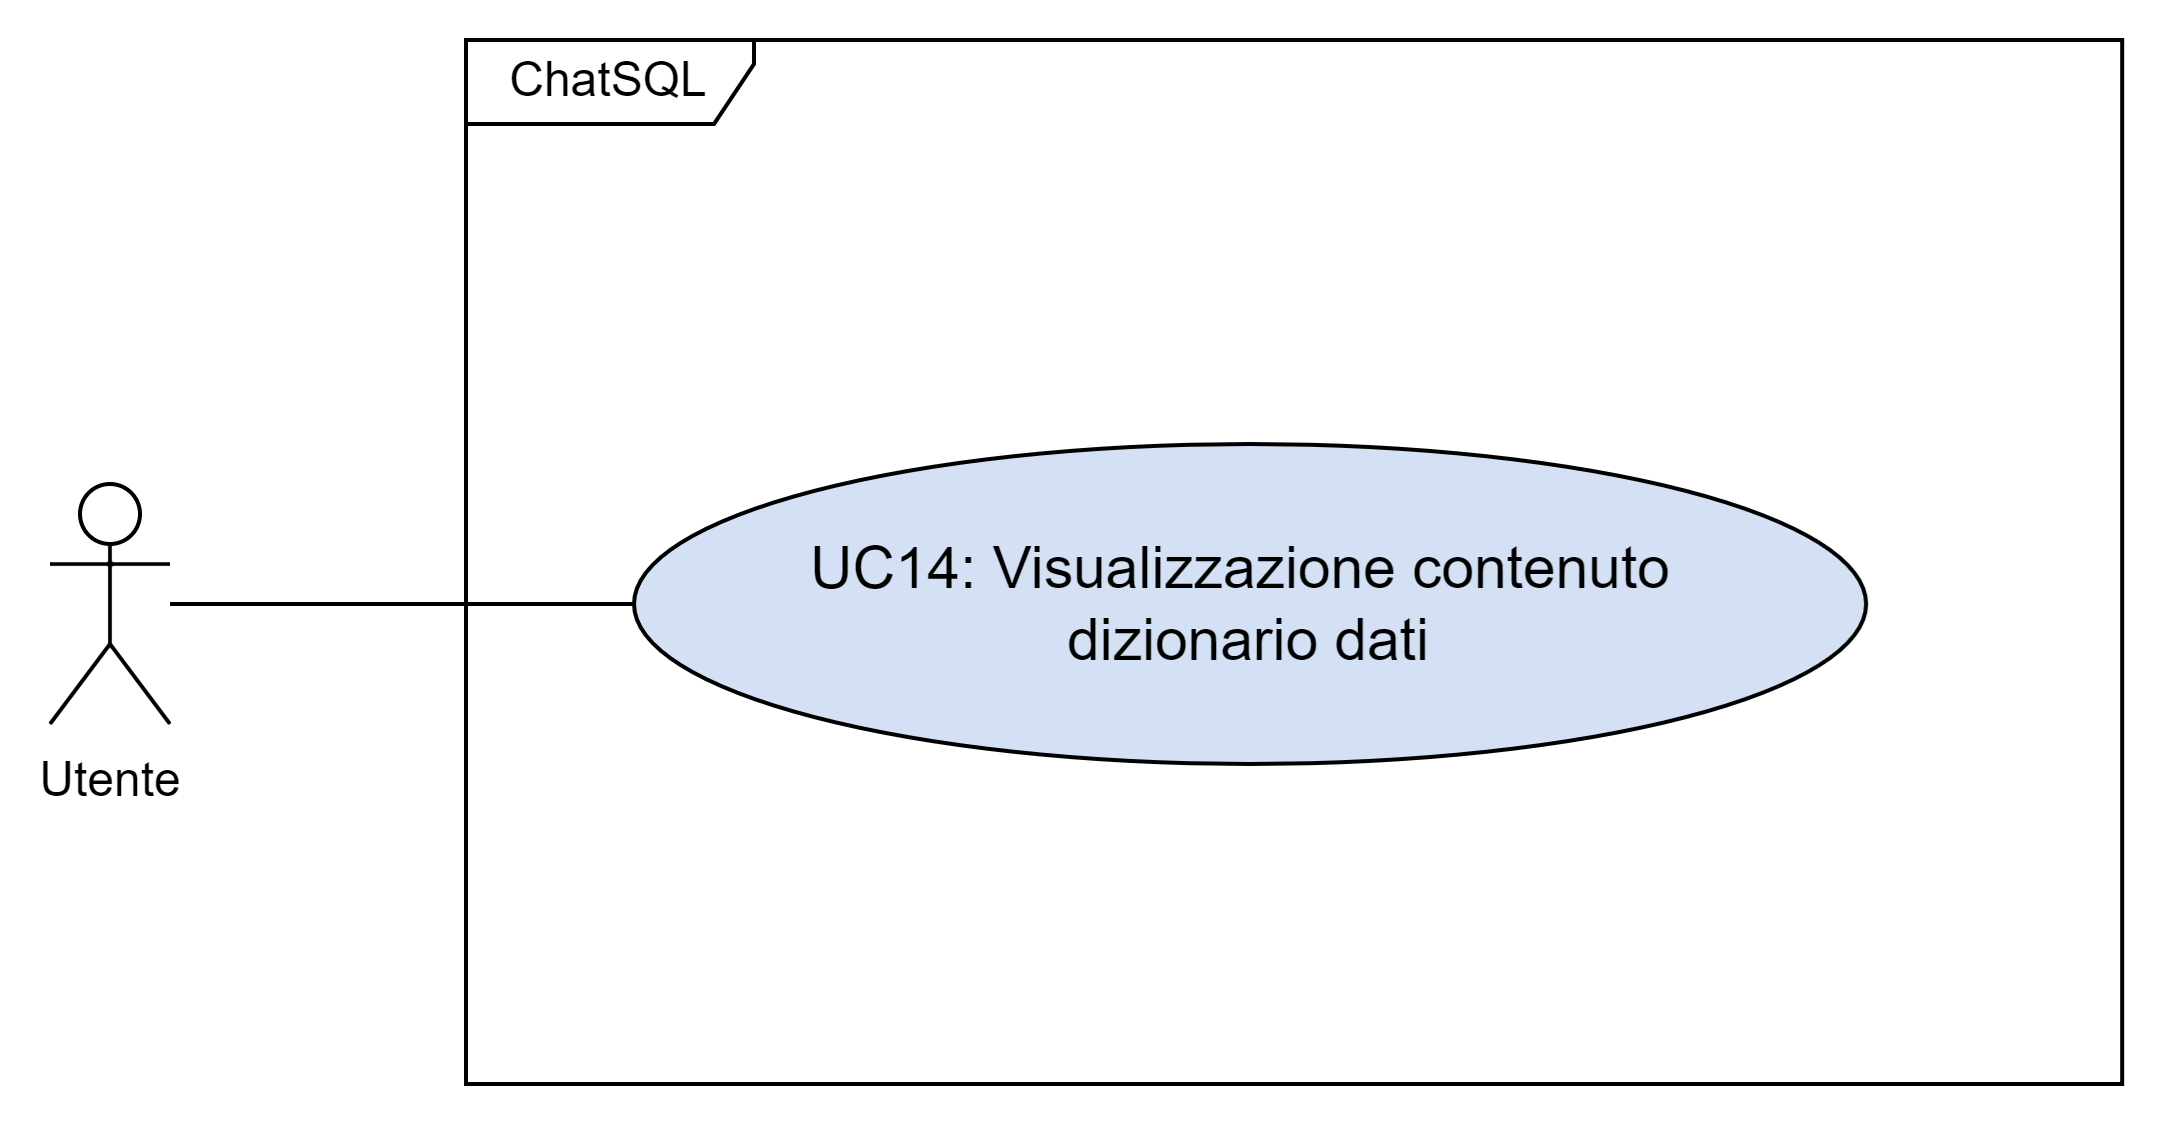
\includegraphics[width=0.90\textwidth]{assets/uc14.png}
  \caption{UC14}
\end{figure}

\paragraph*{Descrizione}
L'Utente visualizza il contenuto del \glossario{dizionario dati} selezionato. Questo comprende la lista delle tabelle e delle colonne, il titolo del \glossario{database} rappresentato dal dizionario e le descrizioni in linguaggio naturale. La visualizzazione del contenuto del dizionario dati può aiutare l'Utente a formulare la richiesta per il \glossario{modello}.

\paragraph*{Attori principali}
Utente

\paragraph*{Precondizioni}
\begin{itemize}
  \item Il sistema è attivo e funzionante;
  \item È presente almeno un \glossario{dizionario dati};
  \item L'Utente ha selezionato un \glossario{dizionario dati} (\hyperref[UC4]{UC4});
\end{itemize}

\paragraph*{Postcondizioni}
\begin{itemize}
  \item Vengono visualizzati correttamente i dati del \glossario{dizionario dati} scelto.
\end{itemize}

\paragraph*{Trigger}
L'Utente vuole visualizzare il contenuto di un \glossario{dizionario dati} con l'obiettivo di formulare una richiesta opportuna al ChatBOT.

\paragraph*{Scenario principale}
\begin{enumerate}
  \item L'Utente seleziona un \glossario{dizionario dati} (\hyperref[UC4]{UC4});
  \item L'Utente visualizza le informazioni contenute nel dizionario.
\end{enumerate}

\paragraph*{Inclusioni}
\begin{itemize}
  \item Visualizzazione tabelle del dizionario (\hyperref[UC14point1]{UC14.1});
  \item Visualizzazione descrizione e sinonimi delle tabelle (\hyperref[UC14point2]{UC14.2});
  \item Visualizzazione sinonimi delle colonne (\hyperref[UC14point3]{UC14.3});
\end{itemize}

%%%%%%%%%%%%%%%%%%%%%%%%%%%%%%%%%%%%%%%%%%%%%%%%%%%%%%%%%%%%%%%%%%%%%%%%%%%%%%

% Da definire i sottocasi